\documentclass[tikz,border=3pt]{standalone}
\usepackage{amsmath,amssymb}
\usepackage{xcolor}
\usetikzlibrary{arrows.meta,calc,positioning}

% colors (approx.)
\definecolor{cGreen}{HTML}{28A745}
\definecolor{cBlue}{HTML}{007BFF}
\definecolor{cOrange}{HTML}{F39C12}
\definecolor{cRed}{HTML}{E74C3C}
\definecolor{cPurple}{HTML}{7D3C98}

\tikzset{
  gridlines/.style={draw=black!50, line width=0.4pt},
  bbox/.style={draw=black, very thick},
  arr/.style={line width=1.2pt, -{Stealth[length=2.5mm, width=2.2mm]}},
}

% one-line helper
\newcommand{\rowline}[3]{%
  \draw[arr, #2] (0,#1) -- (5,#1);
  \node[anchor=west] at (5.4,#1) {$j(4,#1)=#3$};
}

\begin{document}
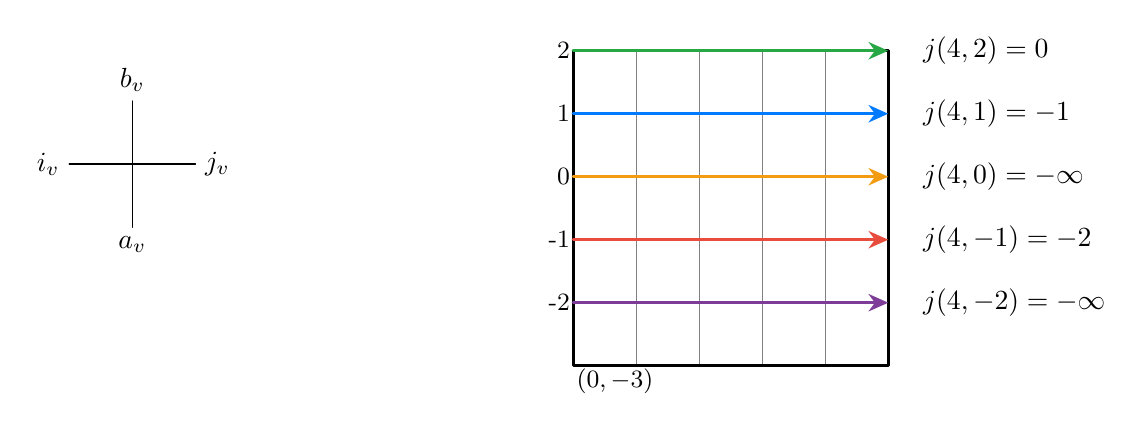
\begin{tikzpicture}[x=0.8cm,y=0.8cm,line cap=round,line join=round]

  %---------------- Left panel: cross with labels ----------------%
  \begin{scope}[shift={(0,0)}]
    \draw[line width=0.6pt] (-1,0)--(1,0);
    \draw[line width=0.6pt] (0,-1)--(0,1);
    \node[below] at (0,-1) {$a_v$};
    \node[above] at (0, 1) {$b_v$};
    \node[left]  at (-1,0) {$i_v$};
    \node[right] at ( 1,0) {$j_v$};
  \end{scope}

  %---------------- Right panel: grid + colored rows -------------%
  % move the right panel to the right
  \begin{scope}[shift={(7.0,-0.2)}] % adjust horizontal spacing if needed
    % grid rectangle and inner grid lines
    \draw[gridlines, step=1] (0,-3) grid (5,2);
    \draw[bbox] (0,-3) rectangle (5,2);

    % y tick labels on the left edge
    \foreach \yy in {-2,-1,0,1,2}{
      \node[anchor=east, inner sep=1pt] at (0,\yy) {\small \yy};
    }
    % bottom-left corner coordinate
    \node[anchor=north west, inner sep=1pt] at (0,-3) {\small $(0,-3)$};

    % colored horizontal arrows and RHS text
    \rowline{ 2}{cGreen}{0}
    \rowline{ 1}{cBlue}{-1}
    \rowline{ 0}{cOrange}{-\infty}
    \rowline{-1}{cRed}{-2}
    \rowline{-2}{cPurple}{-\infty}
  \end{scope}

\end{tikzpicture}
\end{document}